\chapter{Introduction}
\section{first section}
This is the introduction Figure \ref{fig:my_label}.

Now reference an eqn about linear algebra: \eqref{eq:Linear Algebra}.
\begin{figure}
    \centering
    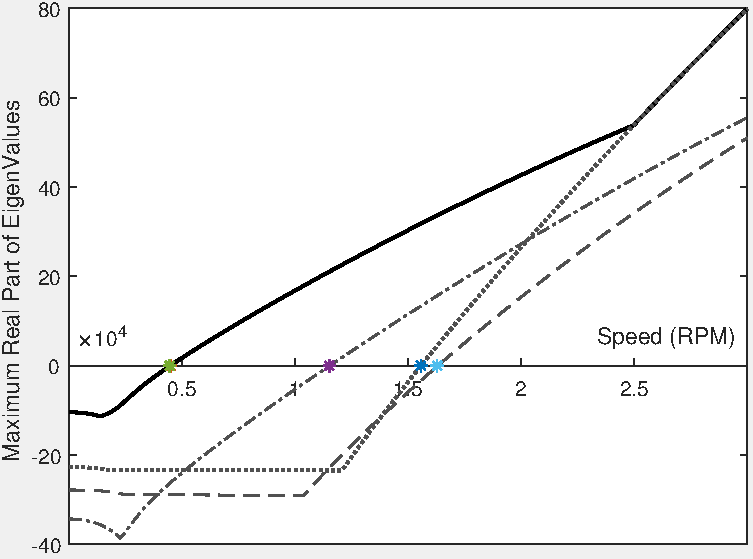
\includegraphics[width=\linewidth]{figures/StabilityMargin.pdf}
    \caption{Caption}
    \label{fig:my_label}
\end{figure}
\begin{equation} \label{eq:Linear Algebra}
\underline{A}\vec{x}=\underline{B}
\end{equation}
\lstinputlisting[language=Matlab]{code/Add.m}
% Matlab Figure%%%%%%%%%%%%%%%%%%%%%%
\begin{figure}
	
	\tikzset{every picture/.style={scale=.8}}%
	\centering
	\import{figures/}{test1.tex}
	\caption{Free body diagram of a beam section in planar bending.}
	\label{fig:test1}
\end{figure}
% Inkscape Figure%%%%%%%%%%%%%%%%%%%%%
\begin{figure}
	\centering
	\def\svgwidth{400pt}
	\import{figures/}{BeamElement.pdf_tex}
	\caption{Beam Element with nodal displacements.}
	\label{fig:BeamElem}
\end{figure}